\documentclass[a4paper, 12pt]{article}

% Paquetes
\usepackage[utf8]{inputenc}
\usepackage[spanish, es-nolayout,es-nodecimaldot,es-tabla]{babel}
\usepackage{amsmath}
\usepackage{amsfonts}
\usepackage{amssymb,amsthm}
\usepackage{enumerate}
\usepackage{enumitem}
\usepackage{parskip}
\usepackage{nicefrac}
\usepackage[left=2cm,right=2cm,top=2cm,bottom=1cm]{geometry}
\usepackage[colorlinks = true]{hyperref}
\usepackage{graphicx}

\newtheorem{teo}{Teorema}

% Comandos
\newcommand{\R}{\mathbb{R}}
\newcommand{\yds}{\qquad\text{y}\qquad}
\DeclareMathOperator{\proy}{proy}
\DeclareMathOperator{\dd}{d}
\linespread{1.25}


% Informativos
\parindent = 0mm
\author{Kerly Naranjo}
\title{Capítulo 6 Tarea 6}
\date{\today}
  

% Contenido
\begin{document}
	\maketitle
	La solución de la ecuación diferencial
	\begin{align*}
	  y^{'}(x)+2y(x)&= 
	  \begin{cases}
	1&  \text{si} \quad x \in [0,3], \\
	%x(n), & \text{si} \quad n \leq -1 \\
	0& \text{si} \quad x \textgreater 3 ; \\	 	
	\end{cases}
	\\ 
	\text{sujeto a}\quad \quad &\\
	 y(0)&=0\\
	\end{align*}
	esta dada por la función a trozos 
	\[
	 y(x) = \begin{cases}
	\dfrac{1}{2}(e^{-2x}-1)&  \text{si} \quad x \leq 3,
	\\
	\\    
    \dfrac{1}{2}(e^{-2x}-e^{6-2x})& \text{si}\quad x   \textgreater 3.
	 \\	 	
	\end{cases}
     \]
\begin{center}
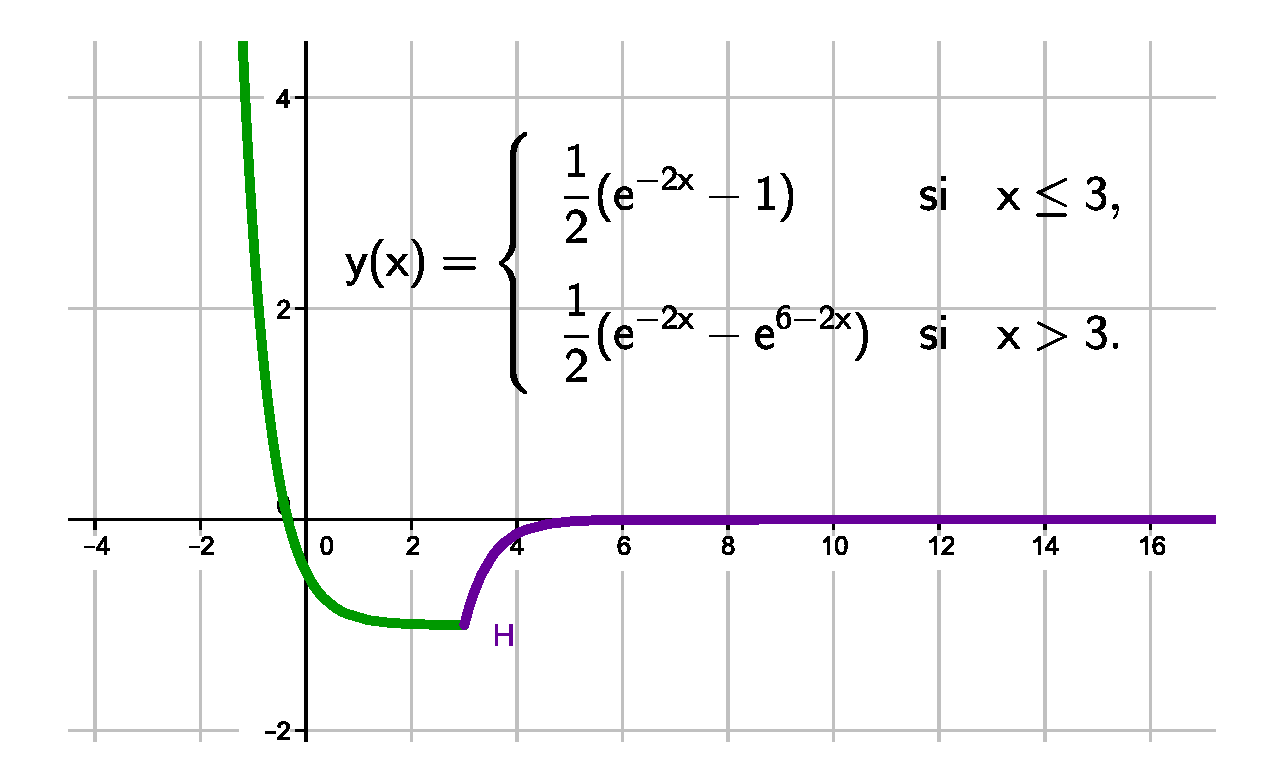
\includegraphics[scale=0.5]{figure1.pdf}
\end{center}

\end{document}